\documentclass[10pt,landscape,a4paper]{article}
\usepackage[utf8]{inputenc}
\usepackage[ngerman]{babel}
\usepackage[T1]{fontenc}
%\usepackage[LY1,T1]{fontenc}
%\usepackage{frutigernext}
%\usepackage[lf,minionint]{MinionPro}
\usepackage{tikz}
\usetikzlibrary{shapes,positioning,arrows,fit,calc,graphs,graphs.standard}
\usepackage[nosf]{kpfonts}
\usepackage[t1]{sourcesanspro}
\usepackage{multicol}
\usepackage{wrapfig}
\usepackage[top=2mm,bottom=4mm,left=2mm,right=2mm]{geometry}
\usepackage[framemethod=tikz]{mdframed}
\usepackage{microtype}
\usepackage{pdfpages}
\usepackage{xcolor}
\usepackage{soul}
\usepackage{graphicx}
\usepackage{caption}
\usepackage{tabularx}
\usepackage{amsmath}
\usepackage{xspace}

\definecolor{myblue}{RGB}{0, 0, 255} % 中等亮度的蓝色
\definecolor{myorange}{RGB}{255, 165, 0} % 较深的橙色
\definecolor{mypurple}{RGB}{128, 0, 128} % 中等亮度的紫色
\definecolor{mygreen}{RGB}{0, 128, 0} % 深绿色
\definecolor{lightblue}{RGB}{173, 216, 230}   % 浅蓝色
\definecolor{lightorange}{RGB}{255, 218, 185} % 浅橙色
\definecolor{lightpurple}{RGB}{221, 160, 221} % 浅紫色
\definecolor{lightgreen}{RGB}{144, 238, 144}  % 浅绿色

\newcommand{\hlblue}[1]{{\sethlcolor{lightblue}\hl{#1}}}
\newcommand{\hlorange}[1]{{\sethlcolor{lightorange}\hl{#1}}}
\newcommand{\hlpurple}[1]{{\sethlcolor{lightpurple}\hl{#1}}}
\newcommand{\hlgreen}[1]{{\sethlcolor{lightgreen}\hl{#1}}}


\let\bar\overline

\definecolor{myblue}{cmyk}{1,.72,0,.38}

\def\firstcircle{(0,0) circle (1.5cm)}
\def\secondcircle{(0:2cm) circle (1.5cm)}

\colorlet{circle edge}{myblue}
\colorlet{circle area}{myblue!5}

\tikzset{filled/.style={fill=circle area, draw=circle edge, thick},
    outline/.style={draw=circle edge, thick}}
    
\pgfdeclarelayer{background}
\pgfsetlayers{background,main}

\everymath\expandafter{\the\everymath \color{myblue}}
\everydisplay\expandafter{\the\everydisplay \color{myblue}}

% \renewcommand{\baselinestretch}{.8}
% \pagestyle{empty}

% \global\mdfdefinestyle{header}{%
% linecolor=gray,linewidth=1pt,%
% leftmargin=0mm,rightmargin=0mm,skipbelow=0mm,skipabove=0mm,
% }

\newcommand{\header}{
\begin{mdframed}[style=header]
\footnotesize
\sffamily
AIAA 5028 Cheat Sheet\\
Zhao Xu, Siqi Lai, Ziyang Wu
\end{mdframed}
}
% \newcommand{\header}{}
\makeatletter % Author: https://tex.stackexchange.com/questions/218587/how-to-set-one-header-for-each-page-using-multicols
\renewcommand{\section}{\@startsection{section}{1}{0mm}%
                                {.2ex}%
                                {.2ex}%x
                                {\color{myblue}\sffamily\small\bfseries}}
\renewcommand{\subsection}{\@startsection{subsection}{1}{0mm}%
                                {.2ex}%
                                {.2ex}%x
                                {\sffamily\bfseries}}

\newcommand{\ie}{\emph{i.e.,}\xspace}
\newcommand{\eg}{\emph{e.g.,}\xspace}
\newcommand{\etc}{\emph{etc.}\xspace}
\newcommand{\etal}{\emph{et al.}\xspace}

\def\multi@column@out{%
   \ifnum\outputpenalty <-\@M
   \speci@ls \else
   \ifvoid\colbreak@box\else
     \mult@info\@ne{Re-adding forced
               break(s) for splitting}%
     \setbox\@cclv\vbox{%
        \unvbox\colbreak@box
        \penalty-\@Mv\unvbox\@cclv}%
   \fi
   \splittopskip\topskip
   \splitmaxdepth\maxdepth
   \dimen@\@colroom
   \divide\skip\footins\col@number
   \ifvoid\footins \else
      \leave@mult@footins
   \fi
   \let\ifshr@kingsaved\ifshr@king
   \ifvbox \@kludgeins
     \advance \dimen@ -\ht\@kludgeins
     \ifdim \wd\@kludgeins>\z@
        \shr@nkingtrue
     \fi
   \fi
   \process@cols\mult@gfirstbox{%
%%%% START CHANGE
\ifnum\count@=\numexpr\mult@rightbox+2\relax
          \setbox\count@\vsplit\@cclv to \dimexpr \dimen@-1cm\relax
\setbox\count@\vbox to \dimen@{\vbox to 1cm{\header}\unvbox\count@\vss}%
\else
      \setbox\count@\vsplit\@cclv to \dimen@
\fi
%%%% END CHANGE
            \set@keptmarks
            \setbox\count@
                 \vbox to\dimen@
                  {\unvbox\count@
                   \remove@discardable@items
                   \ifshr@nking\vfill\fi}%
           }%
   \setbox\mult@rightbox
       \vsplit\@cclv to\dimen@
   \set@keptmarks
   \setbox\mult@rightbox\vbox to\dimen@
          {\unvbox\mult@rightbox
           \remove@discardable@items
           \ifshr@nking\vfill\fi}%
   \let\ifshr@king\ifshr@kingsaved
   \ifvoid\@cclv \else
       \unvbox\@cclv
       \ifnum\outputpenalty=\@M
       \else
          \penalty\outputpenalty
       \fi
       \ifvoid\footins\else
         \PackageWarning{multicol}%
          {I moved some lines to
           the next page.\MessageBreak
           Footnotes on page
           \thepage\space might be wrong}%
       \fi
       \ifnum \c@tracingmulticols>\thr@@
                    \hrule\allowbreak \fi
   \fi
   \ifx\@empty\kept@firstmark
      \let\firstmark\kept@topmark
      \let\botmark\kept@topmark
   \else
      \let\firstmark\kept@firstmark
      \let\botmark\kept@botmark
   \fi
   \let\topmark\kept@topmark
   \mult@info\tw@
        {Use kept top mark:\MessageBreak
          \meaning\kept@topmark
         \MessageBreak
         Use kept first mark:\MessageBreak
          \meaning\kept@firstmark
        \MessageBreak
         Use kept bot mark:\MessageBreak
          \meaning\kept@botmark
        \MessageBreak
         Produce first mark:\MessageBreak
          \meaning\firstmark
        \MessageBreak
        Produce bot mark:\MessageBreak
          \meaning\botmark
         \@gobbletwo}%
   \setbox\@cclv\vbox{\unvbox\partial@page
                      \page@sofar}%
   \@makecol\@outputpage
     \global\let\kept@topmark\botmark
     \global\let\kept@firstmark\@empty
     \global\let\kept@botmark\@empty
     \mult@info\tw@
        {(Re)Init top mark:\MessageBreak
         \meaning\kept@topmark
         \@gobbletwo}%
   \global\@colroom\@colht
   \global \@mparbottom \z@
   \process@deferreds
   \@whilesw\if@fcolmade\fi{\@outputpage
      \global\@colroom\@colht
      \process@deferreds}%
   \mult@info\@ne
     {Colroom:\MessageBreak
      \the\@colht\space
              after float space removed
              = \the\@colroom \@gobble}%
    \set@mult@vsize \global
  \fi}

\makeatother
\setlength{\parindent}{0pt}

\begin{document}

%\footnotesize
\small
\begin{multicols*}{5}
% \fontsize{7pt}{4.5pt}\selectfont
\fontsize{6pt}{4pt}\selectfont

\textcolor{myblue}{test}
\textcolor{myorange}{test}
\textcolor{mypurple}{test}
\textcolor{mygreen}{test}
\hl{Lecture 1}
\hlgreen{outline}
\hlorange{knowledge point}
\hlblue{examples}
\hlpurple{emphasize}


\hl{L1} Network refers to real systems; graph: a mathematical representation of a network, $G=(V,E)$. $e_{ij}\in E$ (directional) relationship between $v_i$ and $v_j$. 
\hlorange{Bipartite graph}$V=V_1 \cap V_2, v_i \in V_1, v_j \in V_2 \text{for all } e_{ij} \in E$.(user-item interactions recommender system).
\hlorange{Heterogeneous graph}$G=(V,E,R,T), r_{ij} \in R$ relation type, $T(v_i)$ node type
\hlorange{hypergraph} \( \mathcal{G} = (V, E, W) \), an edge \( e_j \) can connect any number of vertices, \( W_j \) denotes the weight of the hyperedge. 
\hlorange{dynamic graph} \( \mathcal{G}^t = (V^t, E^t) \), via sequentially updating \( \mathcal{G}^0 \) temporal events \( S = \{s_{t_1}, \dots, s_{t'}, \} \) happened before \( t \).  (transaction graph).
\hlorange{adjacent matrix, adjacency list} adjList[0] will have all the nodes which are connected (neighbour) to vertex 0 and so on. 
\hlorange{tasks} Node-level tasks tasks associated with individual nodes (traffic forecastting rs as v, connectivity as e). edge-level refer to tasks associated with a pair of nodes (Recommender sys). Graph-level tasks Infer if a molecular can be used as antibiotics. 
\hlorange{Unsupervised learning} aims to learn a mapping function without supervision signals to discover underlying patterns.
\hlorange{Semi-supervised learning} aims to learn an input-output mapping function based on partial supervision signals.


\hl{L2} \hlgreen{Traditional Graph Mining Approaches}: Step 1: Deign effective handcrafted features for node, link, graph level tasks by hand and prior.Step 2: Extract features and ML model training. 
\hlorange{Walk} is an alternating sequence of nodes and edges, starting with a node and ending with a node where each edge is incident with the nodes immediately preceding and following it.
\hlorange{Path} is a walk whose nodes are distinct. 
\hlorange{Connected component}. Given a graph \( \mathcal{G} = (V, E) \), a subgraph \( \mathcal{G}' = (V', E') \) is said to be a connected component if there is at least one path between any pair of nodes, and the nodes in \( V' \) are not adjacent to any vertices in \( V \setminus V' \).
\hlorange{Shortest path} \( p_{st\text{min}} = \arg\min |p| \) where \( p \) denotes the path with length \( |p| \). there could be more than one shortest path between any given pair of nodes.
\hlorange{Diameter} a connected graph \( \mathcal{G} = (V, E) \), \( \text{D}(\mathcal{G}) = \max_{v, w \in V} \min|p| \) max length of the shortest path
\hlorange{Complete graph} whose degree \( L = L_{\text{max}} \), and average degree is \( \langle k \rangle = N - 1 \).
    The maximum number of links a network of \( N \) nodes can have is:
    \( L_{\text{max}} = \binom{N}{2} = \frac{N(N - 1)}{2} \), average degree<k>=N-1
\hlorange{scale-free graph} most real-world graphs are sparse and follow power law distribution\({\mathbb  {P}}(d=k)\propto {\frac  {1}{k^{{\gamma }}}}\) \( \gamma \) is a parameter with \( 2 < \gamma < 3 \).
\hlgreen{Node level feature} node centrality Measure the importance of a node in a graph, ie, Node degree. \hlorange{Eigenvector centrality} the node’s centrality is proportional to the average centrality of its neighbors The eigenvector centrality can be rewritten as
\(c_v = \frac{1}{\lambda} \sum_{u \in N} A_{uv} c_u\)
\( c \) is the eigenvector and \( \lambda \) is the maximum eigenvalue. \( \lambda \mathbf{c} = A \mathbf{c} \) The centrality score is the eigenvector of \( A \). 
\hlblue{eg} The largest eigenvalue is 2.482 and its corresponding eigenvector is [1, 0.675, 0.675, 0.806, 1], where the degree of \(v_2, v_3, v_4\) are 2, but the eigenvector centrality of \(v_4\) is higher since it directly connected to \(v_1\) and \(v_5\), whose eigenvector centrality is higher.
 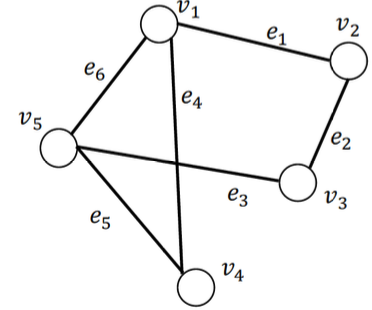
\includegraphics[height=0.025\textwidth]{figs/l2-4.png}
 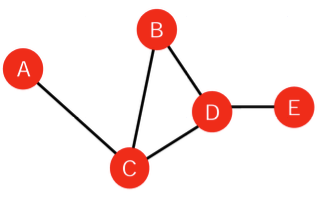
\includegraphics[height=0.025\textwidth]{figs/l2-5.png}
\hlorange{betweenness centrality} \(c(v) = \frac{\sum_{s,t \in V} \sigma_{st}(v)}{\sigma_{st}}\)
where \( \sigma_{st} \) denotes the total number of shortest paths from \( v_s \) to \( v_t \), and \( \sigma_{st}(v) \) indicates the number of these paths passing through \( v \). \hlblue{eg} \(c_A=c_B=c_E=0, c_C=c_D=3 (A-\underline{C}-B, A-\underline{C}-D, A-\underline{C}-D-E)\)
\hlorange{Clustering coefficient} The proportion of closed triangles in a node’s local neighborhood
\(c_u = \frac{\left| (v_1, v_2) \in E : v_1, v_2 \in N(u) \right|}{((d_u \times (d_u - 1) / 2 )} \)
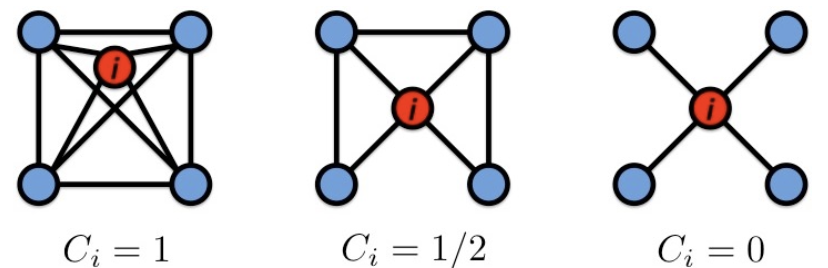
\includegraphics[height=0.025\textwidth]{figs/l2-1.png}
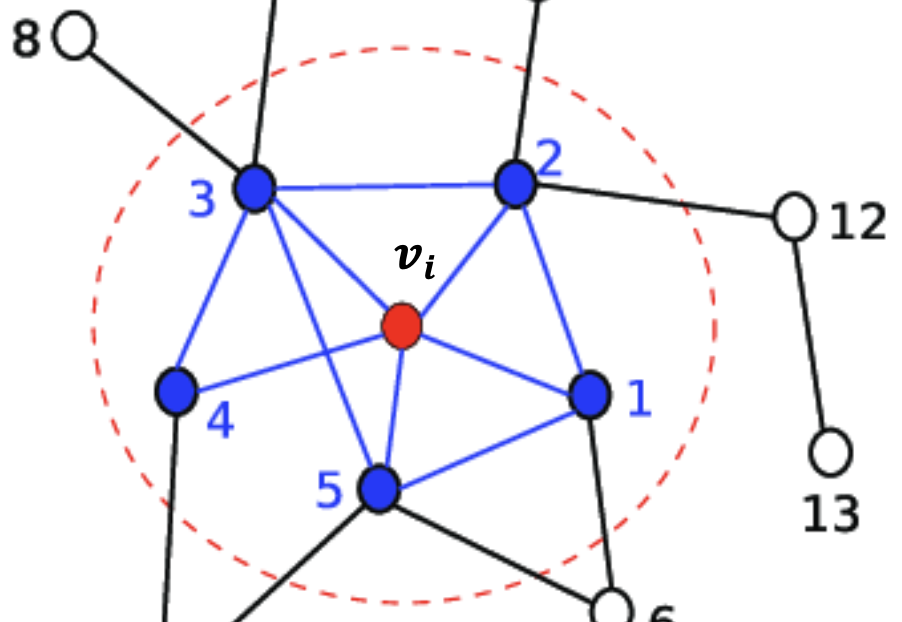
\includegraphics[height=0.025\textwidth]{figs/l2-2.jpg}
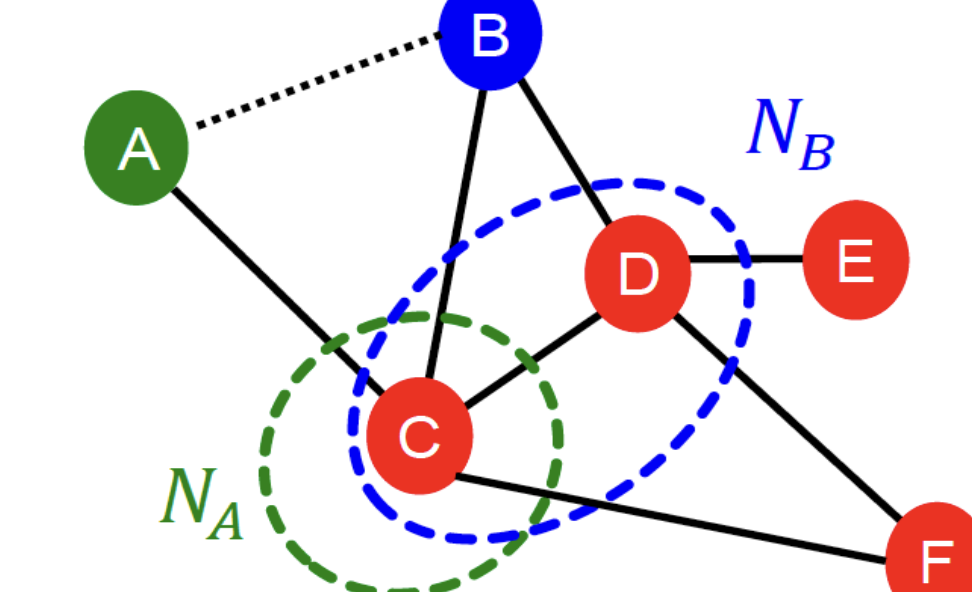
\includegraphics[height=0.025\textwidth]{figs/l2-3.png}
\hlorange{structure-based coefficient}Ego graph a subgraph that contains that node v, its neighbors, and all the edges between v and its neighborhood. 
\hlorange{Motifs and graphlets} Extends from triangles to more complex. \hlorange{limitation of node level feature} fail to encode the relationship between pair of nodes
\hlgreen{Link level feature: local neighbor overlap} \hlorange{shortest path distance} limitation: the topology between two nodes, overlap of neighbors, is overlooked.
\hlorange{Common neighbors:}\( S_c = |N(v_1) \cap N(v_2)| \)
\( S_c = 1 \)
\hlorange{Jaccard overlap:}
\(S_j = \frac{|N(v_1) \cap N(v_2)|}{|N(v_1) \cup N(v_2)|}\) 
\( S_j = \frac{1}{2} \)
\hlorange{Adamic-Adar index:}
\(S_AA = \sum_{v \in N(v_1) \cap N(v_2)} \frac{1}{\log(|N(v)|)}\) 
\( S_AA = \frac{1}{log4} \)
\hlgreen{global neighbor overlap}Limitation of local overlap: fail to handle node pairs without common neighbors.
\hlorange{Katz index}: count the number of paths of all lengths between a given pair of nodes \(S_katz=\sum_{i=1}^{\infty}\beta^i A^i[u,v]\), closed form \(S=(I-\beta A)^{-1} - I\), \(\beta\) discount factor, \(A^i[u,v]\) \# of walks length i between u and v.
\hlorange{Random walk feature} measure how likely we are to reach u from v via random walks.
\() S_{rw} = q_{u}[v] + q_{v}[u]\), \( q_{u} = (1 - c)(I - cP)^{-1} e_{u}\), \( e_{u} \) is the one-hot indicator vector for \( u \), \( P = AD^{-1} \) via personalized PageRank.
\( q_{u}[v]\) gives the stationary probability that random walk starting at node \( u \) visits node \( v \).
\hlgreen{graph kernel methods}
\hlorange{Weisfeiler-Lehman Kernel}
\hlorange{graph level featureLimitation}: overlook important global properties.
1. Assign initial label (color) \( l^0(v) \) to each node, e.g., based on node degree 
\( l^0(v) = d_v, \quad \forall v \in V \)
2. Iteratively update label by hashing current labels within the node’s neighborhood 
\( l^i(v) = \text{HASH}\left(\{ l^{i+1}(u) \, \forall u \in N(v) \}\right) \)
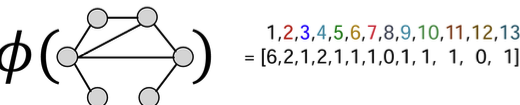
\includegraphics[height=0.025\textwidth]{figs/l2-8.png}
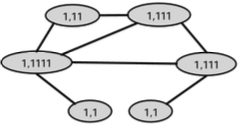
\includegraphics[height=0.02\textwidth]{figs/l2-6.png}
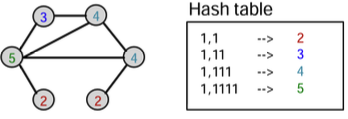
\includegraphics[height=0.025\textwidth]{figs/l2-7.png}
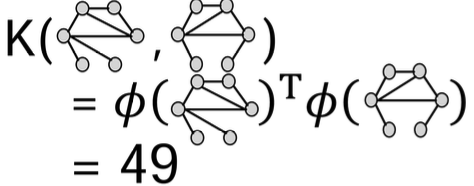
\includegraphics[height=0.025\textwidth]{figs/l2-9.png}
\hlorange{Graphlets Kernel} the distribution of small subgraph structures in the graph. but WL kernel is more efficient $O(\left|E\right|)$, and graphlet is $O(n^k)$ k is the size of graphlets.
\hlgreen{Spectral Graph Theory}
\hlorange{graph signal} \(u_i^TLu_i, u_i^TLu_0 = \lambda_0=0, u_i^TLu_1=\lambda_1, ...\)


\hl{L3:NetworkEmbedding} 
\hlgreen{NE: Node}Project nodes in a unified vector space to preserve the network similarity. Workflow of Learning NE: \hlpurple{encoder} projects nodes to embeddings; Define the \hlpurple{similarity} function for network structures Euclidean/Cosine distance; \hlpurple{decoder} recover; Optimize parameters to minimize the reconstruction loss.
$L = \sum_{u,v \in \mathcal{D}} \ell( \mathrm{DEC}(z_u, z_v),\mathrm{Similarity}(u,v))$
\hlorange{homogeneous or heterogeneous} In a homogeneous graph, all the nodes represent instances of the same type and all the edges represent relations of the same type. in a heterogeneous graph, the nodes and edges can be of different types.
\hlgreen{NE: node relationship} \hlpurple{co-occurrence}: random walk; \hlpurple{proximity}(nearness in space, time, or relationship.): 1st,2nd order.
\hlpurple{word2vec} maximize the probability of co-occurrence of close words for each word.
\hlorange{random walk: Advantages} 
\hlpurple{Expressivity:} Flexible stochastic definition of node similarity that incorporates both local and higher-order neighborhood information. If a random walk starting from node \( u \) visits \( v \) with high probability, \( u \) and \( v \) are considered similar (this reflects high-order multi-hop information).
\hlpurple{Efficiency:} Do not need to consider all node pairs when training; consider pairs that co-occur on random walks.
\hlblue{EG: v1-v2-v3-v4-v5-v6} 
\begin{tabular}{|c|c|}
\hline
\textbf{node} & \textbf{context nodes} \\
\hline
$v1$ & $v2,v3$ \\
$v2$ & $v1,v3,v4$ \\
$v3$ & $v1,v2,v4,v5$ \\
$v4$ & $v2,v3,v5,v6$ \\
\hline
\end{tabular} 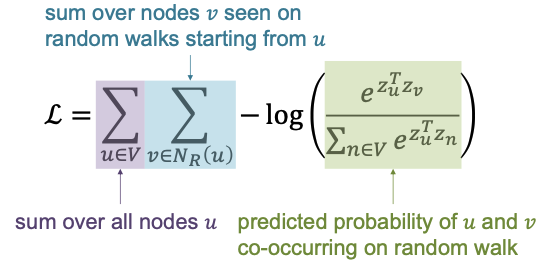
\includegraphics[height=0.045\textwidth]{figs/l3-1.png}
\hlorange{deepwalk} predict the context nodes with embedings, Maximize conditional probability:\(p(v_{context} | v_{cen})\)
\hlorange{Limitation:} Nested sum over all nodes results in \( O(|V^{2}|) \) complexity.
\hlorange{Negative Sampling}
\(L=-\log\left(\frac{\exp(\mathbf{z_u^T z_v})}{\sum_{n \in V} \exp(\mathbf{z_u^T z_n})}\right) \approx \log\left(\sigma(\mathbf{z_u^T z_v})\right) + \sum_{i=1}^{k} \log\left(\sigma(-\mathbf{z_u^T z_{n_i}})\right)\) 
% \textcolor{red}{spend more time} 
another way to improve efficiency is 
\hlorange{Hierarchical Softmax}: optimize embeddings with Hierarchical Softmax using Stochastic Gradient Descent.
\hlorange{Node2Vec} difference between deepwalk: Develop biased second order random walk  \(\mathcal{R}\) to generate network neighborhood  \(\mathcal{N}_0(u) \text{ of node } u.\)
\hlorange{Biased walks:}
To trade off between local and global views of the network.
1. Local view: visited through BFS. (purple)
2. Global view: visited through DFS. (orange)
\hlorange{N-order Proximity} First order proximity: for two nodes connected by edge. Second order proximity: for 2-hop neighbor. Optimize two decoder separately using KL-divergence. node 6, 7: 1st order; node 6, 5 2nd order. dtx is the distance from t to x.
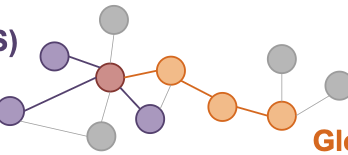
\includegraphics[height=0.03\textwidth]{figs/l3-4.png}
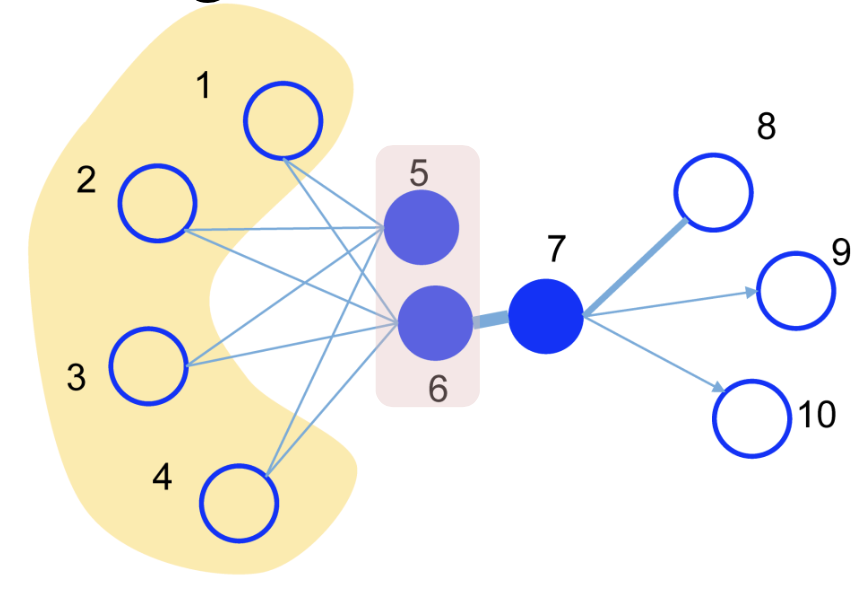
\includegraphics[height=0.03\textwidth]{figs/l3-2.png}
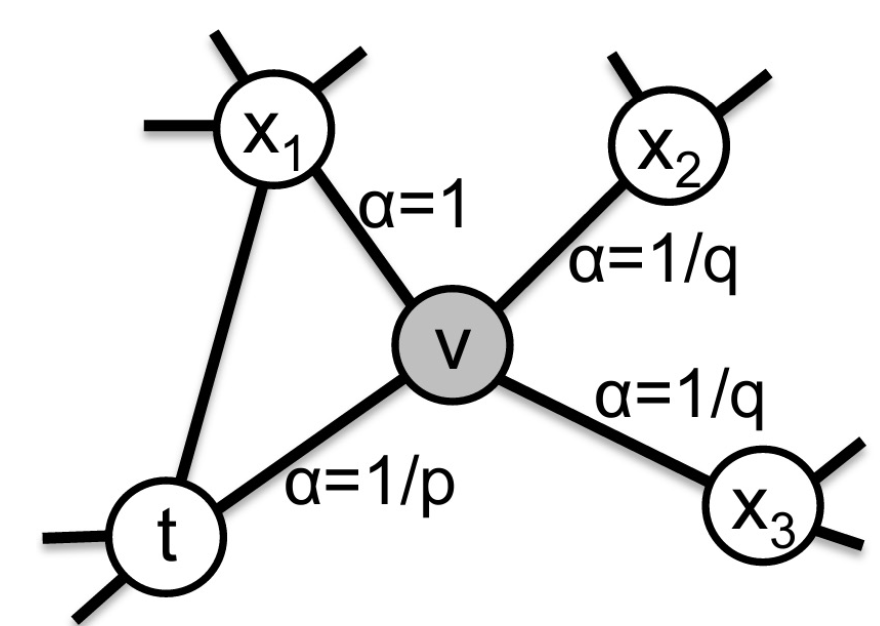
\includegraphics[height=0.03\textwidth]{figs/l3-3.png}
\(a_{pq}(t, x) = 
\begin{cases} 
\frac{1}{p} & \text{if } d_{tx} = 0 \\
1 & \text{if } d_{tx} = 1 \\
\frac{1}{a} & \text{if } d_{tx} = 2 \\
\end{cases}
\)
Smaller p result in sampled neighbors around t (BFS), smaller q result in sampled neighbors away from t (DFS)
\hlgreen{NetworkEmbedding: structural relationship} preserving structural feature: Microscopic and Mesoscopic.
\hlorange{struc2vec}preserve microscopic node similarity. Suppose u v are two distant nodes; They are structural similar, but hard to measure. 1. Measure structural role similarity g(vi, vj); 2. build a new graph; 3. deep walk -> node embedding.
\hlorange{Modularized Nonnegative Matrix Factorization (M-NMF)} preserve mesoscopic community structure.
Exploit the consensus relationship between the representations of nodes and community structure.
Joint optimization: a. NMF based representation learning model; b. Modularity based community detection model.
\hlorange{summary}Network embedding on simple networks: preserving node/structure based similarity. Preserving \hlpurple{node} relationship: DeepWalk, Node2Vec; Preserving \hlpurple{structure} information: Microscopic (close neighbors): Struc2Vec; Mesoscopic (community): M-NMF

\hl{L4:GNN1} \hlpurple{RELU}\(f(x) = \max(0, x)\) \hlpurple{Sigmoid}\(f(x) = \frac{1}{{1 + e^{-x}}}\)
\hlorange{Feedforward Neural Networks for graph}Problem: 1. Problems:O(|V|) parameters, 2.Not applicable to graphs of different sizes 2. Sensitive to node ordering
\hlorange{CNN for graph}Problem: 1. Problems: 1. There is no notion of sliding window on graph. 2. CNNs are sensitive to input size and order, whereas graphs are variable in size and permutation invariant. 
\hlorange{Permutation Invariance and Permutation Equivariance} FNNs, CNNs, are Not permutation invariant / equivariant! Graph Neural Networks should be permutation invariant and equivariant. Given arbitrary order plan, equivariant same as the order plan, invariant as the whole graph. Then, if \( f(Ai,Fi) = f(Aj,Fj) \) for any order plan \( i \) and \( j \), we formally say \( f \) is a \hlpurple{permutation invariant} function. If the output vector of a node at the same position in the graph remains unchanged for any order plan, we say f is \hlpurple{permutation equivariant}
\hlorange{Framework for Node level tasks} a composition of graph convolution and non-linear activation layers
\hlorange{Framework for Graph level tasks} graph convolution and pooling layer (Summarize node features to generate the representation for the subgraphs or the entire graph).



\hl{L5:GNN2}
\hlgreen{graph convolution}
\hlorange{Laplacian matrix} For a given graph \( g = (V, E) \) with \( A \) as its adjacency matrix, its Laplacian matrix is defined as \( L = D - A, \) where \( D \) is a diagonal degree matrix \( \text{diag}(d_{v1}, \dots, d_{v_2}) \) 
% \textcolor{red}{Eigen-decomposition of Laplacian Matrix}
Laplacian matrix is a difference operator:
\( h = Lf = (D - A)f = Df - Af \quad (f \in \mathbb{R}^{n \times 1}) \)
\( h(i) = \sum_{ v_j \in N(v_i)}(f(i) - f(j)) \quad  \)
Laplacian quadratic form: \( f^T L f = \frac{1}{2} \sum_{i,j=1}^{N} A[i,j](f(i) - f(j))^2 \)
\hlorange{Spectral-Based Graph Convolution}  First apply Graph Fourier Transform (GFT) on the graph to obtain its Graph Fourier coefficients, and then modulate these coefficients before reconstructing the signal in the spatial domain. the graph filters can be learned.
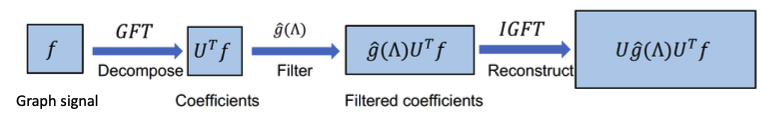
\includegraphics[height=0.02\textwidth]{figs/l5-1.png}
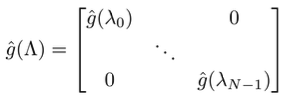
\includegraphics[height=0.018\textwidth]{figs/l5-2.png}
\hlorange{limitations of Primal Graph Filter:} 1. \# of learned parameters is equal to \# of nodes N; 2. convolution operator is not spatially localized; 3. eigen decomposition of the Laplacian matrix is computational expensive.
\hlorange{Polynomial Filter Operator}Spectral Decomposition:
\(
\mathbf{L} = \mathbf{U} \mathbf{\Lambda} \mathbf{U}^T
\)
k-order Polynomial Filter Operator:
\(
g(\mathbf{\Lambda}) = \sum_{k=0}^{K} \theta_k \mathbf{\Lambda}^k
\), 
\(f'= \mathbf{U} g(\mathbf{\Lambda}) \mathbf{U}^T \mathbf{f}
= \sum_{k=0}^{K} \theta_k \mathbf{U} \mathbf{\Lambda}^k\mathbf{U}^T f=\sum \theta_kL^kf
\), 
\(\mathbf{U} \mathbf{\Lambda}^k\mathbf{U}^T = \mathbf{U} (\mathbf{\Lambda}\mathbf{U}^T\mathbf{U})^k\mathbf{U}^T = L^k\)
\hlorange{Limitations of Polynomial Filter} $g(x)=\theta_0 + \theta_1x+\theta_2x^2$ 1. Non-orthogonal; 2. Unstable under perturbation of coefficients
\hlorange{Chebyshev Polynomials} form an orthogonal basis for the Hilbert space
\(
T_0(x) = 1;
T_1(x) = x;
T_k(x)= 2xT_{k-1}( x) - T_{k-2}(x);
g (x) = \theta_0 T_0( x) + \theta_1 T_1( x) + \theta_2 T_2 (x) + \cdots
\), 
\(
\hat{g}(\mathbf{\Lambda}) = \sum_{k=0}^{K} \theta_k T_k(\Tilde{\mathbf{\Lambda}}), \Tilde{\mathbf{\Lambda}}=\frac{2\Lambda}{\lambda_{max}}-1
\),
\(f'= \mathbf{U} \hat{g}(\mathbf{\Lambda}) \mathbf{U}^T \mathbf{f} = \sum_{k=0}^{K} \theta_k T_k(\Tilde{\mathbf{\Tilde{L}}})f, \Tilde{L} =  \frac{2L}{\lambda_{max}}-1\)
\hlorange{GCN: simplified chebNet} K = 1 and $\lambda_{max}=2, \theta=\theta_0=-\theta_1$, \(\hat{g}(\mathbf{\Lambda})=\theta_0 + \theta_1(\Lambda-I) = \theta(2I-\Lambda, \mathbf{U} \hat{g}(\mathbf{\Lambda}) \mathbf{U}^T \mathbf{f}=\theta(2I-L)f=\theta\left(\Tilde{D}^{-\frac{1}{2}}A D^{-\frac{1}{2}} \right)f, \Tilde{A} = A+I \)
\hlorange{Spatial-Based Graph Convolution} \(H^{(l+1)} = \sigma\left(D^{-\frac{1}{2}}A D^{-\frac{1}{2}} H^{(l)} W^{(l)}\right)\) 
spatial-based GNNs including GCN, GraphSAGE and GAT are special cases of Message PassingNN
\hlorange{GraphSAGE} Aggregate: mean, lstm, pool; here is the mean form: \(h_{v}^{(k)} = \sigma\left( W \cdot \text{CONCAT}\left( h_{v}^{(k-1)}, \frac{1}{|\mathcal{N}(v)|} \sum_{u \in \mathcal{N}(v)} h_{u}^{(k-1)} \right) \right)\) $h_{v}^{(k)}$ is the feature representation of node $v$ at the $k^{th}$ layer. $\mathcal{N}(v)$ denotes the set of neighbors of node $v$.
\hlorange{attention} 1. The attention score between a query $q$ and a key $k_i$ is:
\(
\text{score}(q, k_i) = q \cdot k_i^T
\)
2. The attention weights are computed using a softmax over the scores:
\(
\alpha_i = \frac{\exp(\text{score}(q, k_i))}{\sum_{j=1}^{T}\exp(\text{score}(q, k_j))}
\)
3. The attention output is a weighted sum of the values:
\(
\text{Attention output} = \sum_{i=1}^{T} \alpha_i v_i
\)
\hlorange{GAT} The Graph Attention Network (GAT) updates node features based on the following:
% \textcolor{red}{GCN, ChebNet, GAT, GraphSAGE}
1. Compute the attention coefficients between nodes $v$ and $u$:
\(
e_{vu} = \text{LeakyReLU}\left(\mathbf{a}^T [\mathbf{W} \mathbf{h}_v \parallel \mathbf{W} \mathbf{h}_u] \right)
\)
2. Normalize the attention coefficients with softmax:
\(
\alpha_{vu} = \frac{\exp(e_{vu})}{\sum_{k \in \mathcal{N}(v)} \exp(e_{vk})}
\)
3. Update the node features using the normalized attention weights:
\(
h_v' = \sigma \left( \sum_{u \in \mathcal{N}(v)} \alpha_{vu} \mathbf{W} \mathbf{h}_u \right)
\)
where $\mathcal{N}(v)$ denotes the neighbors of node $v$, and $\sigma$ is an activation function.
\hlgreen{Graph Pooling}Flat Graph Pooling and Hierarchical Graph Pooling. 
\hlorange{Flat Graph Pooling } 1. The max-pooling and average pooling operations in classical CNNs can be directly adopted to GNNs. 2. Attention-Based Flat Pooling 1. Compute an attention score for each node:
\(
s_i = \mathbf{a}^T \tanh(\mathbf{W} \mathbf{h}_i)
\)
2. Normalize the scores with softmax:
\(
\alpha_i = \frac{\exp(s_i)}{\sum_{j=1}^{N} \exp(s_j)}
\)
3. Compute the graph representation using the attention weights:
\(
\mathbf{h}_{\text{graph}} = \sum_{i=1}^{N} \alpha_i \mathbf{h}_i
\)
\hlorange{Hierarchical Graph Pooling}  Flat graph pooling ignores the hierarchical sub-graph structure information; Hierarchical graph pooling layers aim to preserve the hierarchical graph structural information by coarsening the graph step by step. 
\hlorange{Downsampling-Based Graph Pooling: gpool}
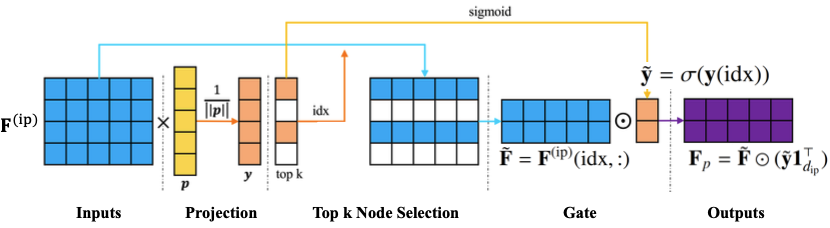
\includegraphics[height=0.022\textwidth]{figs/l5-4.png} 
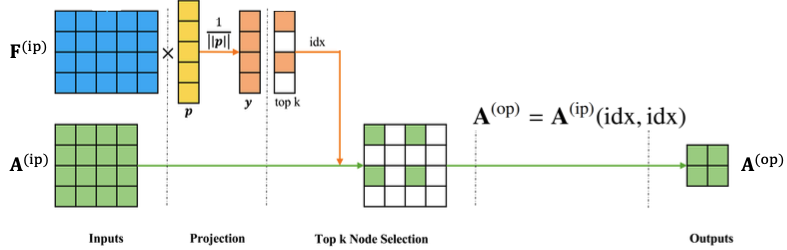
\includegraphics[height=0.022\textwidth]{figs/l5-3.png} 
% \textcolor{red}{Page 65 gPool and DiffPool}
\hlorange{Supernode-Based Graph Pooling: diffpool}
\(S = \text{softmax}(\text{GCN}(A^{ip}, F^{ip}) \in \mathbb{R}^{N_{ip} \times N_{op}}), A^{op}=S^TA^{ip}, F^{op}=S^TGCN(A,F)
\)
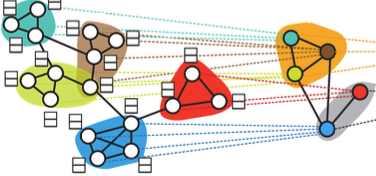
\includegraphics[height=0.022\textwidth]{figs/l5-5.png} 
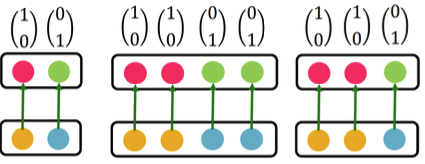
\includegraphics[height=0.022\textwidth]{figs/l6-8.png}
\hl{L6:GNN3} GCN and GraphSAGE’s aggregation functions fail to distinguish some basic multi-sets; hence not injective. GCN (mean-pool): 
$\text{Mean}({f_{u}} n \in N(v)) $
GraphSAGE(max-pool)$\text{Max}({f_{u}} n \in N(v)) $
Function \( g: X \rightarrow Y \) is injective if it maps different elements into different outputs.
\hlorange{Graph Isomorphism Network} 
% \textcolor{red}{formula Page 14 to 25} 
\hlorange{Comparison Between GIN and WL Graph Kernel} 1.Node embeddings are low-dimensional; hence, they can capture the fine-grained similarity of different nodes. 2.Parameters of the update function can be learned for the downstream tasks; 3. Because of the relation between GIN and the WL graph kernel, their expressive is exactly the same. If two graphs can be distinguished by GIN, they can be also distinguished by the WL kernel, and vice versa. 4. \textcolor{blue}{GIN is also powerful enough to distinguish most of the real graphs!}
\hlorange{Improving Expressive Power}GIN and MPNN cannot distinguish some basic graph structures like counting the cycle length. the computation graph for node A and B are same.
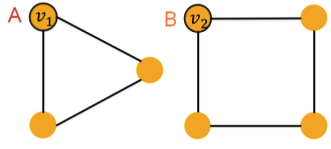
\includegraphics[height=0.02\textwidth]{figs/l6-1.png} 
\hlorange{Position-aware GNNs} 
\hlpurple{Anchors:} 1.Randomly pick node \( s1 \) and \( s2 \) as anchor nodes, which can be used to locate nodes in the graph.2. Represent \( v1 \) and \( v2 \) via their relative distances w.r.t. the anchors
\hlpurple{Anchor sets}1. Generalize anchor from a single node to a set of nodes. 2. We define distance to an anchor-set as the minimum distance to all the nodes in the anchor-set 3. Large anchor-sets provide better position estimation.
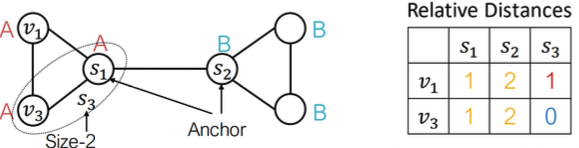
\includegraphics[height=0.03\textwidth]{figs/l6-2.png} How to use position encoding? The simple way: use position encoding as augmented node features (works well in practice). 
\hlpurple{Issue}: if we permute the dimensions of position encoding, the output will change.
\hlpurple{Solution} 1. Sample multiple anchor-sets \( S1 \), \( S2 \), and \( S3 \). 2. For node \( v1 \), aggregate information from anchor-sets \( S1 \), \( S2 \), \( S3 \) to obtain embeddings \( Mv1[1] \), \( Mv2[2] \), \( Mv3[3] \). 3. Aggregate \( Mv1[1] \), \( Mv2[2] \), \( Mv3[3] \) to obtain \( hv1 \) (for next layer) and position embedding \( zv1 \) (for output).
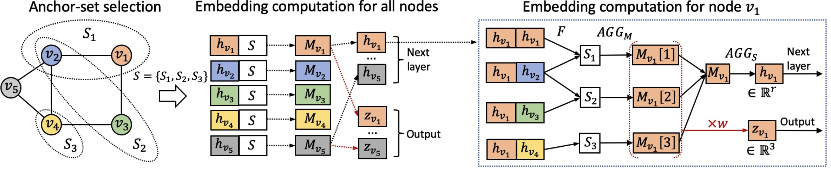
\includegraphics[height=0.035\textwidth]{figs/l6-3.png}
\hlorange{Identity-aware GNNs} Inductive node coloring can help distinguish specific graph structures: Different computational graphs -> successfully differentiate nodes.
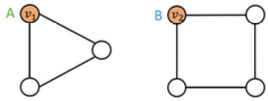
\includegraphics[height=0.025\textwidth]{figs/l6-4.png}
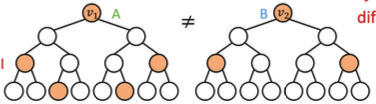
\includegraphics[height=0.025\textwidth]{figs/l6-5.png}
\hlorange{Heterogenous message passing} ID-GNN: at a given layer, different message/aggregation to nodes with different colorings.
\hlorange{Why heterogenous message passing works}1. Suppose two nodes have the same computational
graph, but have different node colorings. 2. Since we apply different neural network for computation, their embeddings will be different.
\hlorange{Summary} 1. ID-GNN is the first message passing framework that is more expressive than 1-WL test. 2. ID-GNN can count cycles originating from a given node, but GNN cannot. 3.ID-GNN can be applied to enhance any message passing GNNs (GCN, GraphSAGE, GIN, ...)
\hlorange{Over-smoothing in GNNs} Stack GNN layers sequentially, which can aggregate multi-hop neighboring nodes. When stacking K-layer GNN, each node has a receptive field of K-hop neighborhood.
\hlorange{Over-smoothing}: all the node embeddings converge to the same value. This is bad because we want to use node embeddings to differentiate nodes. \hlpurple{Reason: } The shared neighbors quickly grows when we increase \# hops (\# GNN layers). Embedding of a node is determined by its receptive field, if two nodes have highly-overlapped receptive fields, then their embeddings are highly similar.
\hlpurple{Solution: }Skip Connection, DropEdge, PairNorm.
\hlorange{Skip Connection} adding shortcuts in GNN. \( N \) skip connections \( \rightarrow \) \( 2^{N} \) possible paths. We automatically get a mixture of shallow GNNs and deep GNNs.
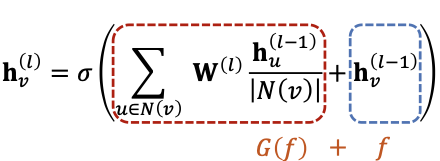
\includegraphics[height=0.025\textwidth]{figs/l6-6.png}
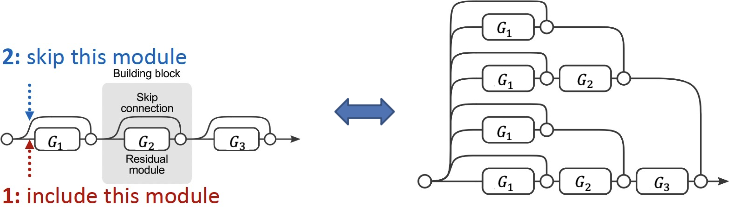
\includegraphics[height=0.025\textwidth]{figs/l6-7.png}
\hlorange{DropEdge }Randomly dropping some edges in the graph during each training epoch
\hlorange{PairNorm} Introduces a regularization term to force representations of nodes that are not connected to be different.

%
% ================ Lexture 7 ================
%
\hl{L7: GNN on Complex Graphs}
\hlorange{\textbf{Heterogeneous graph}}: Graphs have multiple types of nodes and edges. $G=(V,E,R,T)$, where $r_{ij} \in R$ is a relation type, and $t_i \in T$ is a node type.
\hlorange{\textbf{Dynamic graph}}: Graph structure varies with time.
\hlorange{\textbf{Discrete-time dynamic graph (DTDG)}}: Appears in applications with regularly-
sampled data (\eg \hlblue{traffic forecasting}). $[G^{(1)},\dots,G^{(\tau)}]$, where $G^{(t)}=(V^{(t)}, A^{(t)}, X^{(t)})$.
\hlorange{\textbf{Continuous-time dynamic graph (CTDG)}}: $G^t = (V^t, E^t)$, formed via sequentially updating an initial static graph $G^0 = (V^0, E^0)$ according to a set of temporal evolution events $S=\left\{s(t_1),\dots,s(t_n)\right\}$ happened before $t$.
\textcolor{red}{heterogeneity} and \textcolor{red}{temporal dynamics} cannot be captured by classical GNN layers.
\hlorange{\textbf{Heterogeneous network embedding}}: 1) Extract different types of pairs of heterogeneous nodes (\eg \hlblue{(text, image), (text, text)}). 2) Encode each type of node pair using the corresponding weight-sharing module (\eg \hlblue{text by LSTM, image by CNN}). 3) Use a common prediction layer to decode similarity for different relationships.
\hlorange{\textbf{Meta-path}}: A meta-template $\Phi$ in heterogeneous graph $G$ denoted as $(t_1,r_{(1,2)},t_2,\dots,r_{(l-1,l)},t_l)$, where $t_i \in T$ and $r_{i,j} \in R$ are type of the node and the edge (\eg \hlblue{Author-Paper-Author}).
\hlorange{\textbf{$\Phi$-neighbors}}: $N_\Phi(v_i)$ contains nodes that connect with $v_i$ through a meta-path $\Phi$.
\hlorange{\textbf{Heterogeneous Graph Attention Network (HAN)}}:
1) Aggregate information from $\Phi$-neighbors for each $\Phi \in \Psi$ via node-level attention, where $\Psi$ is the set of $P$ meta-path schemes.
% $\alpha^\Phi_{ij}=\frac{exp(\theta(W^T_\Phi\dot[h^\prime_i||h^\prime_j]))}{\sum_{k\in N_\Phi(v_i)} exp(\theta(W^T_\Phi\dot[h^\prime_i||h^\prime_k]))}$
2) Combine the information aggregated from each type of $\Phi$-neighbors through meta-path-level attention (a score for each type) to generate the node representations.
3) Apply the final embedding to supervised tasks and design different loss functions.
\hlorange{\textbf{Heterogeneous Graph Neural Network (HetGNN, Random-walk-based)}}:
1) Sample and select top-$k$ frequent heterogeneous neighbors for each node by Random Walk with Restart (RWR).
2) Extract different types of node contents to generate node content embedding via node heterogeneous contents encoder NN-1.
3) Aggregate embeddings of the sampled heterogeneous neighbors (\ie Type-based neighbor aggregation through NN-2, and Heterogeneous types combination through NN-3).
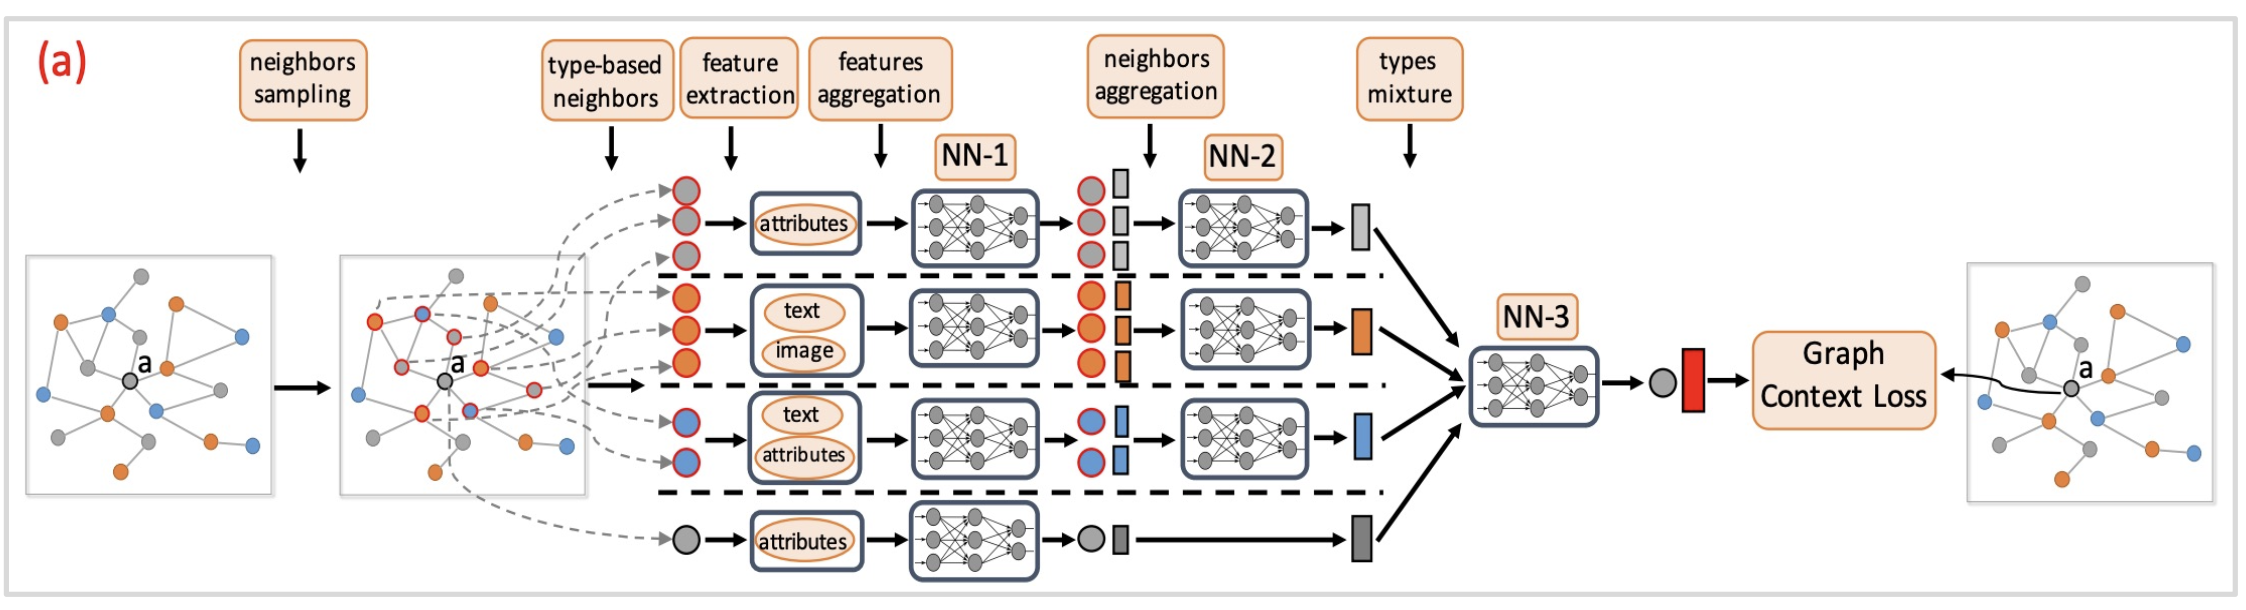
\includegraphics[height=0.052\textwidth]{figs/HetGNN.png}
4) Unsupervised training: Adjacent heterogeneous nodes have similar embeddings. $\mathcal{L}=\sum_{\left \langle v,v_c,v^\prime_c\right \rangle \in T_{walk}} log \sigma(\epsilon_{v_c} \cdot \epsilon_v) + log \sigma (-\epsilon_{v^\prime_c} \cdot \epsilon_v)$, where $\epsilon_v$ is the output embedding, $T_{walk}$ is a set of triplets collected by walk sampling, and $v_c$ is within a distance threshold to $v$ in random walk, and $v^\prime_c$ is a negative node with the same type of $v_c$.
\hlorange{\textbf{Properties of dynamic graphs (DG)}}: 1) Nodes and edges will evolve. 2) Node features and topological structures exhibit temporal patterns.
\hlorange{\textbf{DG evolution types}}: 1) Node and edge addition/deletion. 2) Feature update.
\hlorange{\textbf{DG tasks}}: 1) Extrapolation (\ie predict a future state). 2) interpolation (\ie estimate the past state, like missing value). 3) Time prediction (\ie predict the time for an incoming event).
\hlorange{\textbf{GNN-LSTM for DTDGs}}: 1) Employ a GNN to each graph snapshot $G^t$ and obtain hidden representation $Z^t$. 2) Feed the sequence $[Z^1, \dots,Z^T]$ into LSTM to capture temporal information.
\hlorange{\textbf{EvolveGCN for DTDGs}}: The parameters of GNN at time $t$ are evolved from the model parameters at time $t-1$ by an RNN. $W^{(l-1,t)}=RNN(Z^{(l-1,t)},W^{(l-1,t-1)})$,  $Z^{(l,t)}=GNN(A^{(t)},Z^{(l-1,t)},W^{(l-1,t)})$, where $W^{(l-1,t)}$ are GNN parameters, and $Z^{(l,t)}$ is the GNN output.
\hlorange{\textbf{Joint Dynamic Interaction Embeddings (JODIE) for CTDGs}}: learn dynamic embeddings of each user $u(t)$ and item $i(t)$ at time $t$ from an ordered sequence of temporal user-item interaction events. They use two RNNs to \textcolor{red}{separately} update embeddings of users and items after each interaction. \textcolor{red}{However}, a user’s interests change gradually as time progresses, even without interactions. \textcolor{red}{Therefore}, they predict the future embedding trajectories of users. The model minimizes the $L_2$ distance between the predicted item embedding $\hat{i}(t+\Delta)$ and the real item embedding $i(t^-+\Delta)$ at each interaction. \underline{Limitation}: overlooks the nodes multi-hops away, learns embeddings in a transductive fashion.
\hlorange{\textbf{Temporal Graph Networks (TGN) for CTDGs}}:
1) Memory: stores a state vector $s(t)$ for each node, acting as a condensed representation of all past interactions for each node.
2) Message function: Given an interaction between nodes $i$ and $j$ at time $t$, it two messages ($m_i(t)$ and $m_j(t)$), which are used to update the memory.
3) Memory updater: Aggregate all the messages of node $i$ before time $t$ by an RNN.
4) Graph embedding: Compute the embedding of a node by aggregating the state vector $s(t)$, edge features $e(t)$, and node features $v(t)$ of temporal neighbors. \underline{Staleness problem}: compute embedding of an inactive node by aggregating state vectors of active neighbors.
5) Model training: edge prediction (self-supervised) or node classification (semi-supervised).
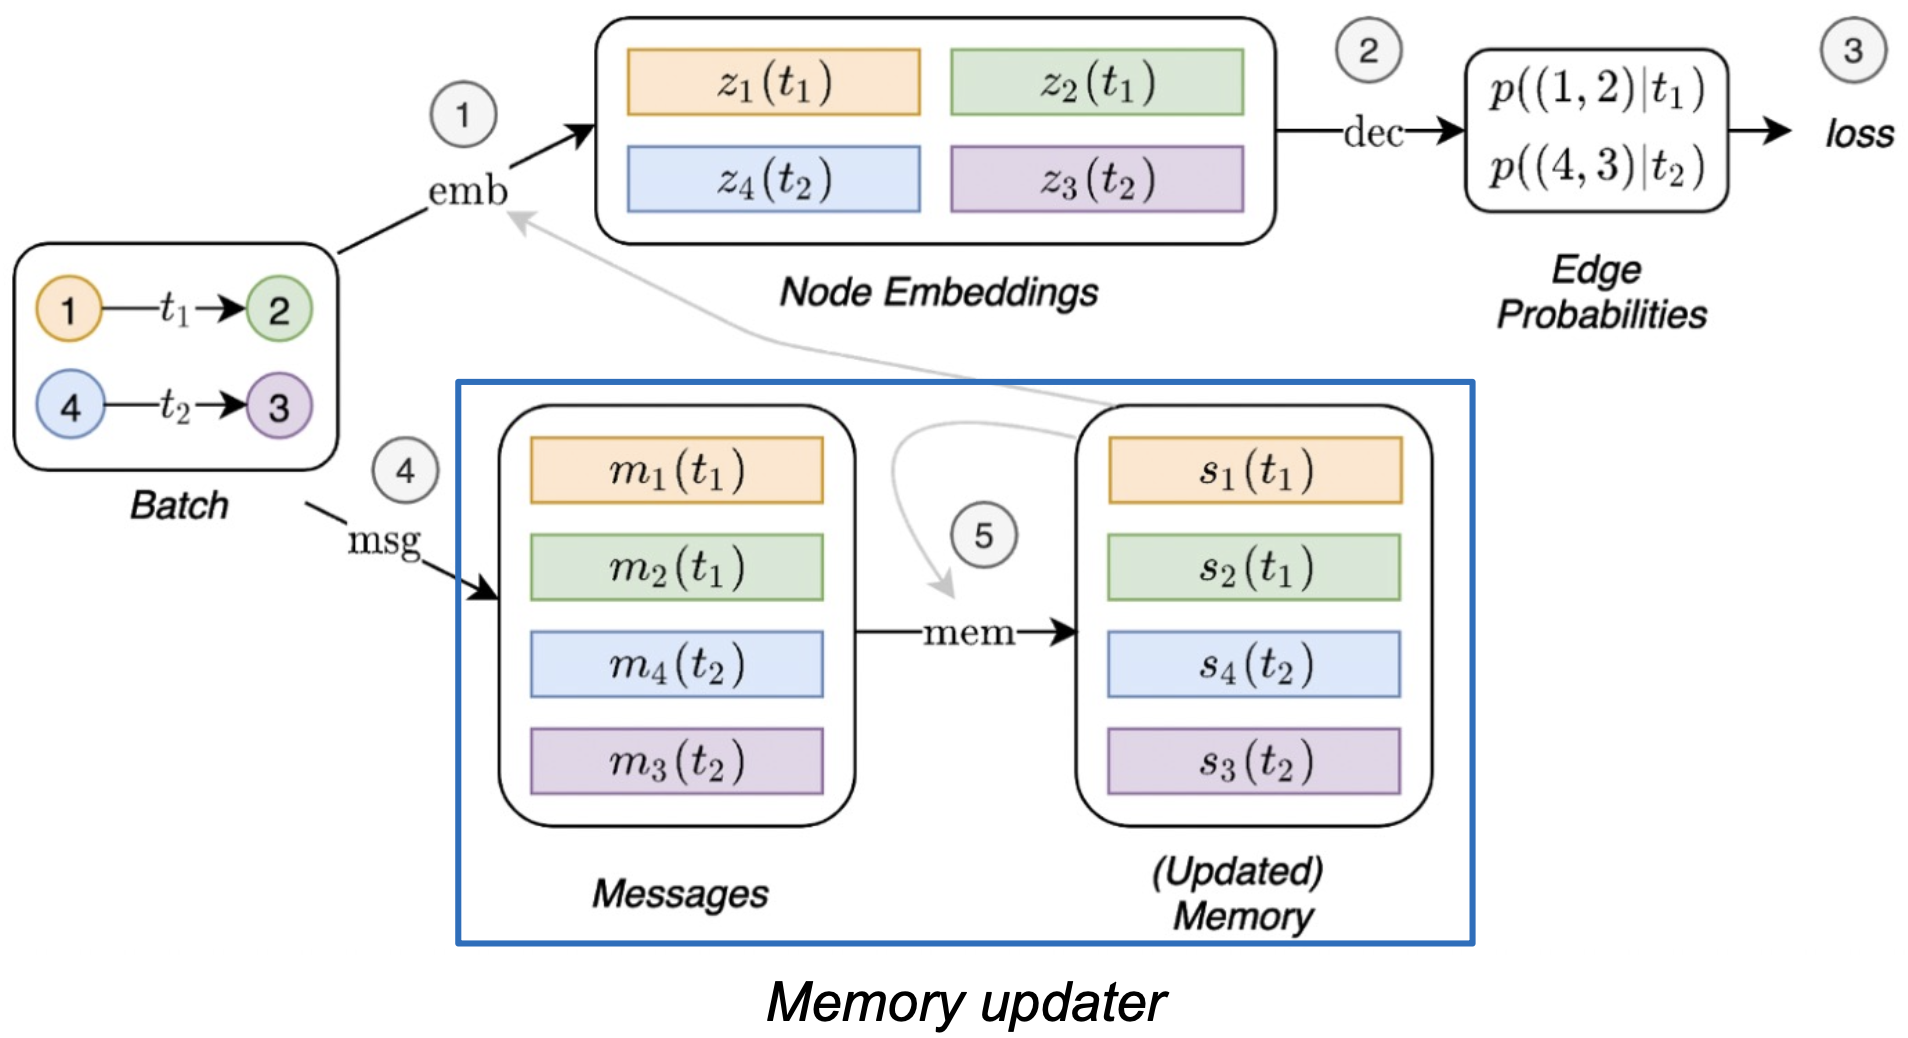
\includegraphics[height=0.07\textwidth]{figs/TGN.png}

%
% ================ Lexture 8 ================
%

\hl{L8: Knowledge Graph}
\hlorange{\textbf{Knowledge Graph (KG)}}: Given a set $\mathcal{E}$ of entities and a set $R$ of relations, a knowledge graph $G$ can be expressed as $G(\mathcal{E}, R, \mathcal{E})$. A triplet  $(h,r,t) \in G$ denotes head entity $h\in \mathcal{E}$ has relation $r \in R$ with tail entity $t\in \mathcal{E}$.
\hlorange{\textbf{KG Applications}}: 1) Link prediction. 2) Triple classification (\ie correct or not). 3) Conversational Recommender Systems.
\hlorange{\textbf{Automatic KG Construction}}:
1) Construct triplets through relationships between entities.
2) Entity and relation embedding: Project entities and relations in the embeddings vector space $R^d$.
3) Representation learning: Given a triple $(h,r,t)$, let $f_r(h,t)=||h+r-t||$ close to 0.
4) Optimization: $\mathcal{L}=\sum_{(h,r,t) \in G}\sum_{(h^\prime,r^\prime,t^\prime) \in G^\prime} (f_r(h,t) - f_r(h^\prime,t^\prime) + \gamma)$, where $\gamma$ is the margin, $G$ are correct triplets, and $G^\prime$ are incorrect ones.
\hlorange{\textbf{KG relation types}}: 1) Symmetric (\eg \hlblue{roommate}). 2) Antisymmetric (\eg \hlblue{teacher}). 3) Inverse (\eg \hlblue{employer and employee}). 4) Composition (\eg \hlblue{My mother's husband is my father}). 5) 1-to-N relations (\eg \hlblue{teacher teaches stu\_1, \dots, stu\_N}).
\hlorange{\textbf{TransE}}: project entities and relations into Euclidean spaces and optimize embeddings by $f_r(h,t)=||h+r-t|| \rightarrow 0$. It \textcolor{red}{can} model 1) Antisymmetric, 2) Inverse, and 3) Composition. But \textcolor{red}{cannot} model 1) Symmetric and 2) 1-N relations.
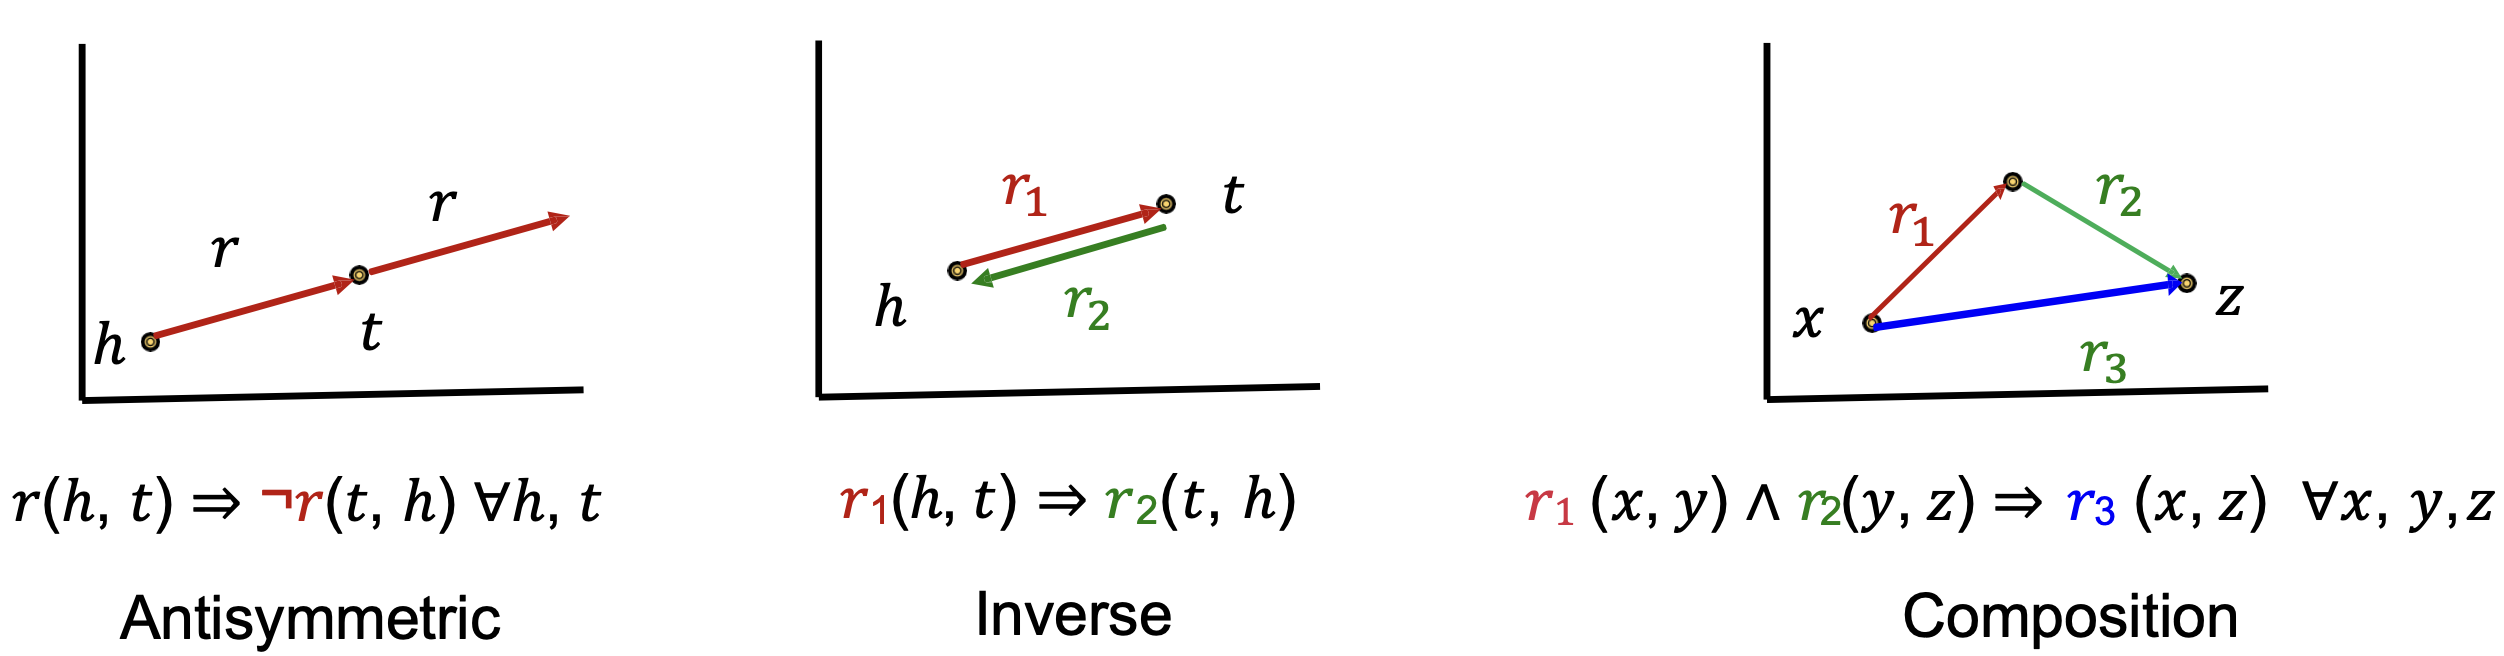
\includegraphics[height=0.05\textwidth]{figs/TransE.png}
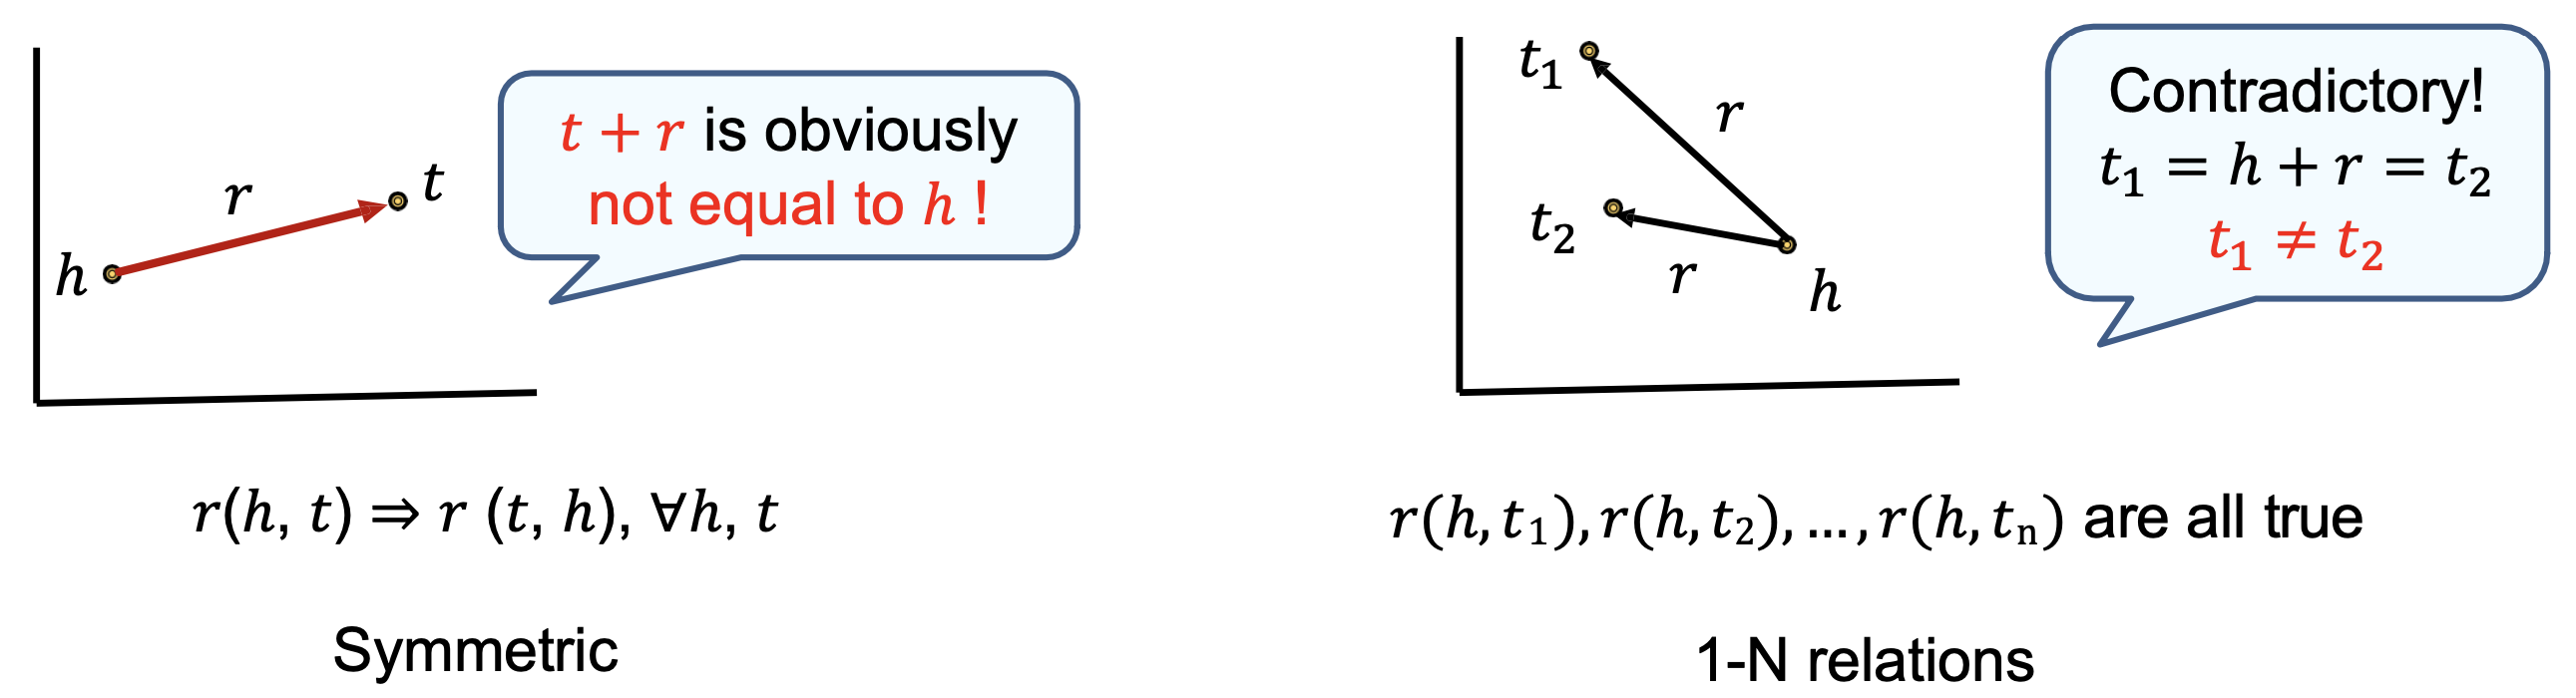
\includegraphics[height=0.05\textwidth]{figs/TransE2.png}
\hlorange{\textbf{TransH}}: Project entity embeddings into relation hyperplanes, TransH \textcolor{red}{can} model 1-N relations. \underline{Project}: $h_\perp=h-W^T_rhW_r$, $t_\perp=t-W^T_rtW_r$, where $W_r$ are learnable parameters. \underline{Score function}: $f_r(h,t)=||h_\perp+r-t_\perp||$.
\hlorange{\textbf{TransR}}: Models entities and relations in entity space and relation spaces, and performs translation in relation space. TransR \textcolor{red}{can} model symmetric and 1-N relations. \underline{Project}: $h_\perp=M_rh$, $t_\perp=M_rt$. \underline{Score function}: $f_r(h,t)=||h_\perp+r-t_\perp||$.
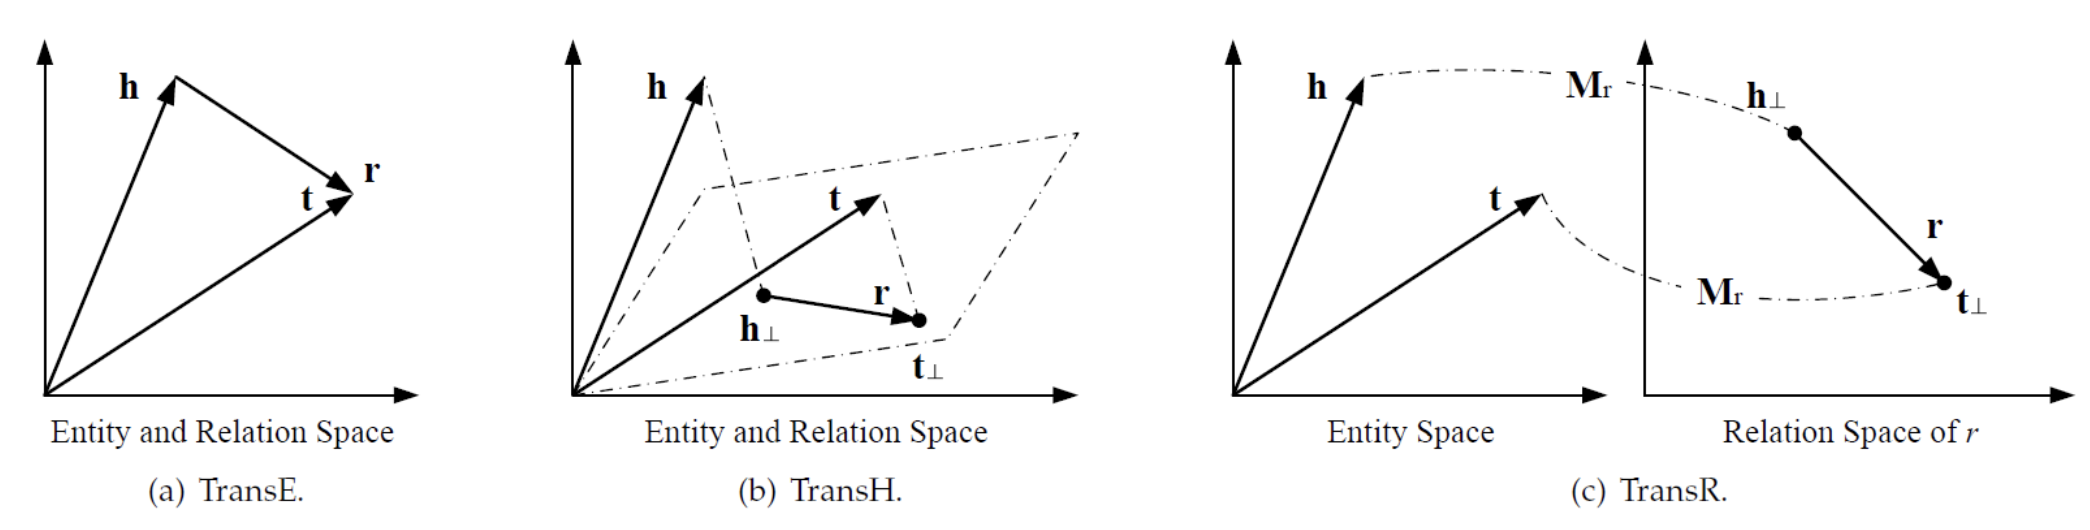
\includegraphics[height=0.05\textwidth]{figs/TransEHR.png}
\hlorange{\textbf{Semantic matching models}}: exploit similarity-based scoring function by neural networks, measuring plausibility of facts by matching \textcolor{red}{latent semantics of entities and relations}.
\hlorange{\textbf{RESCAL}}: \underline{Score function}: $f_r(h,t)=h^T M_r t = \sum^d_i \sum^d_j [h]_i \cdot [M_r]_{ij} \cdot [t]_j$, where $M_r \in R^{d \times d}$ is a matrix associated with the relation.
\hlorange{\textbf{DistMult}}: Simplifies RESCAL by restricting $M_r$ to diagonal matrices. It only captures pairwise interactions between the components of $h$ and $t$ along the \textcolor{red}{same dimension}. \underline{Score functions}: $f_r(h,t)= h^T diag(M_r) t = \sum^d_i [h]_i \cdot [M_r]_i \cdot [t]_i$.
\textcolor{red}{NOTE}: RESCAL and DistMult can only model \textcolor{red}{symmetric} relations.
\hlorange{\textbf{TuckER}}: A KG triplet can be given as a $n\times n \times m$ tensor, where $n$ is number of entities and $m$ is the number of relations. TuckER can decompose the matrix in three directions, obtaining the head entity embeddings, relation embeddings, and tail entity embeddings. \underline{Score function}: $f_r(h,t) = W \times_1 h \times_2 r \times_3 t$, where $\times_n$ indicating the tensor product along the $n^{th}$ mode. TuckER applies logistic sigmoid to each score $f_r(h,t)$ to obtain the predicted probability $p$ of a triplet being true.
\hlorange{\textbf{ConvE}}: 1) Use TransE to get a pre-trained entity and relation embeddings. 2) The entity and relation embeddings are first reshaped and concatenated. 3) The resulting matrix is inputted to a CNN layer. 4) The resulting feature map tensor is projected in a $k$-dimensional space. 5) Calculate the score between $(h, r)$ and $t$ by matching with all candidate tail entity embeddings. \underline{Score function}: $f(vec(f([h,r] * w))W)t$, where $[h,r]$ is the concatenated operation, $w$ is a 2D convolutional filter, and $W$ is a projection matrix.
\hlorange{\textbf{R-GCN}}: Deal with the highly multi-relational data characteristic.
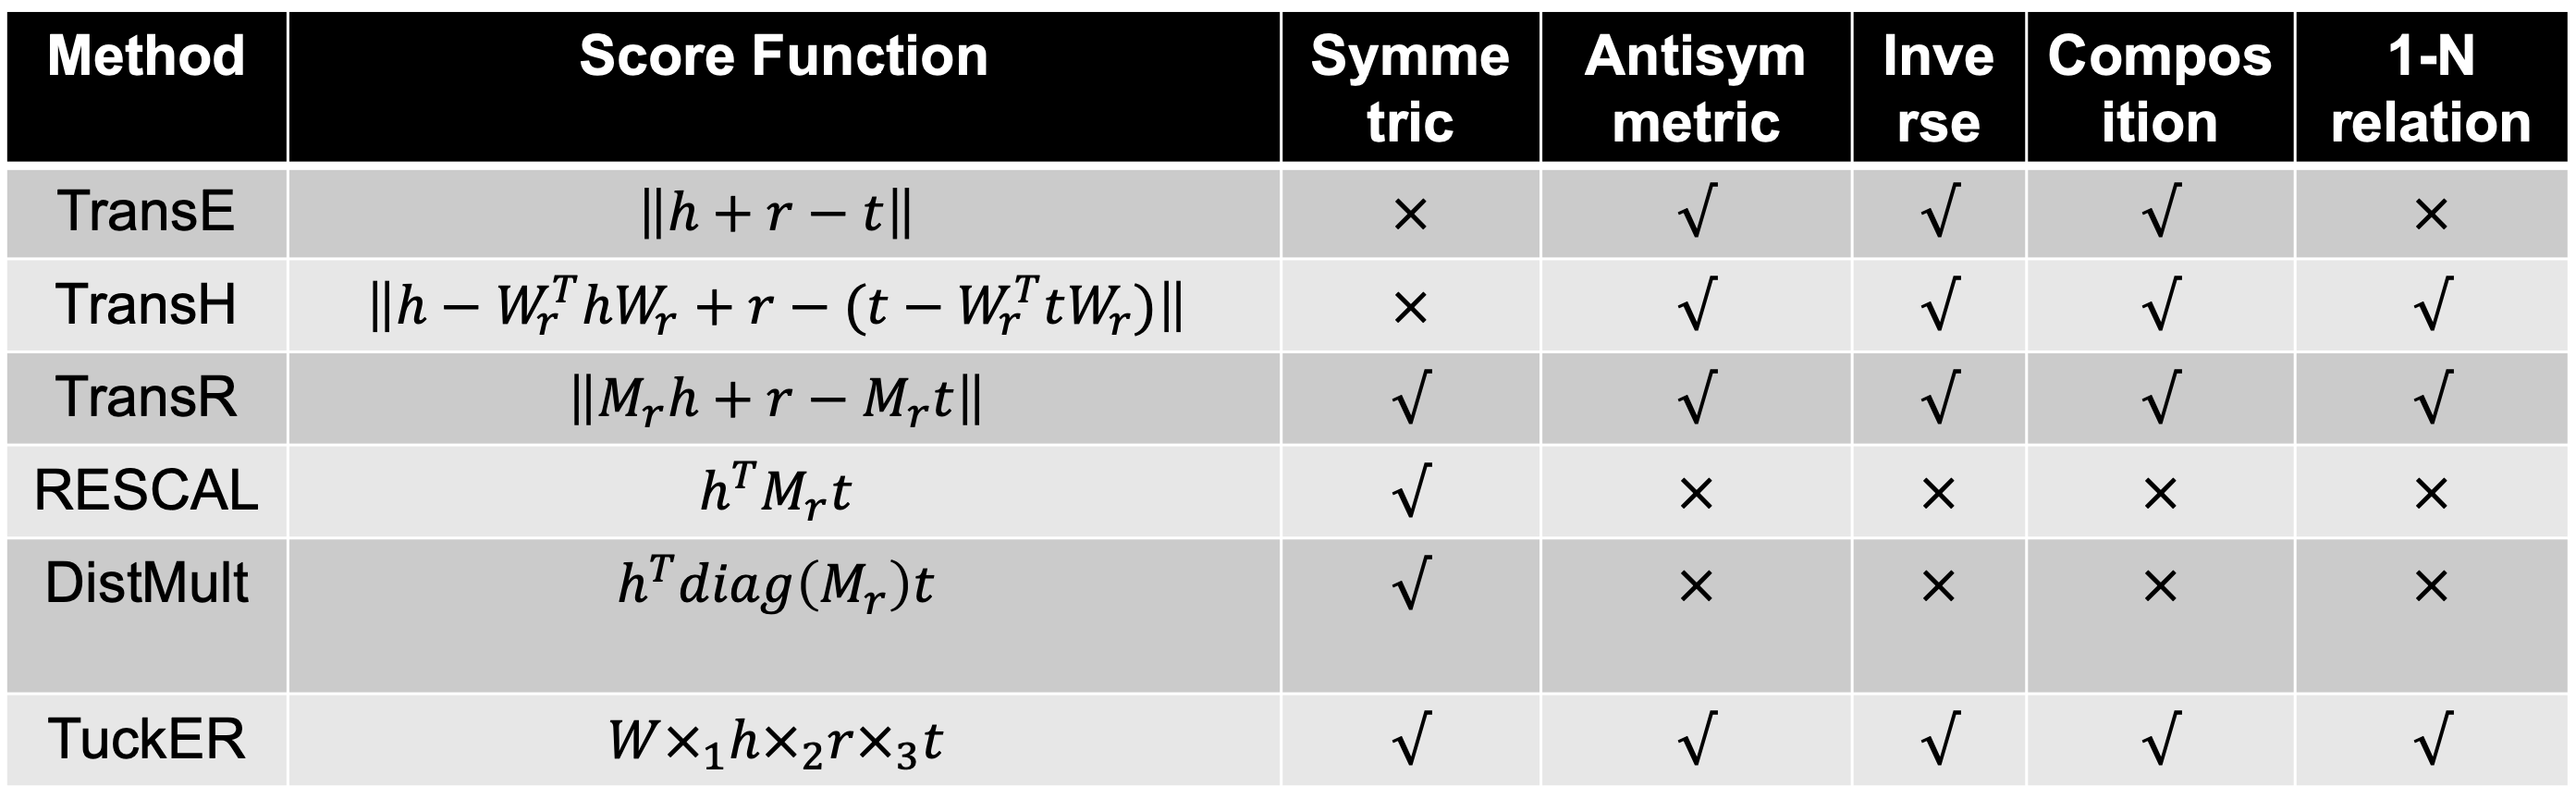
\includegraphics[height=0.06\textwidth]{figs/KGCompare.png}

\hl{L9: ScalableGNN}
Train a GNN in large-scale graph is hard: load the entire graph and features, (1)requiring memory becomes prohibitively large, (2)inefficient gradient update due to minibatch sampling.
\textbf{Three techs:1)Data level: graph sampling, 2)Model level: simplifying GNNs, 3)System level: distributed learning} \hlorange{Graph Sampling}: Cannot sample directly sample nodes because 
it's Necessary to preserve structure information.     \textbf{\textcolor{red}{Node-wise sampling}}: \textbf{Mini-batch training}: Randomly sample a few nodes, leverage computational graph (a node and its neighbor, neighbor's neighbr ...) to aggregate k-hop neighbors, obtaining their embedding and training. \textbf{problem}:neighbor explosion when 1)layer size grows 2)meet high degree nodes. \textbf{GraphSage}:sample neighbors in computational graph. \underline{How to sample?}1) random sample: fast but may sample unimportant nodes. 2) Random Walk with Restarts (
\textcolor{red}{RWR}):Use RWR score to measure the node importance. \underline{Time complexity}: $M*m^K$, M is number of sampled nodes, m is the maximum sampled neighbor number, K is the number of layers. \underline{Limitations}:1) neighbor explosion when m and K are large 2)Smaller m leads to unstable training due to the larger variance in neighbor aggregation. 3)Computation is redundant when nodes in a mini-batch share many neighbors \textbf{GNNAutoScale}: steps: 1)select a mini-batch of nodes,2)only sample one hop (full) neighbors for each node in message passing. (to tackle the issue: GNN may lose out-of-mini-batch information,3)use historical embeddings to approximate the missing out-of-mini-batch information. \underline{Pros}:a)avoid neighborhood
explosion issue, b)low variance c)Reduce redundant computations \underline{Cons}:a)The approximation error leads to performance drop, b) Historical embeddings require CPU memory storage. \textbf{\textcolor{red}{Subgraph-wise Sampling}}: sample small graphs. Motivation: Real-world graph exhibits community structure. Each community retains essential local connectivity patterns of the original graph. \hlorange{Vanilla Cluster-GCN}: First, Use any community detection algorithms (Louvain, METIS) to partition nodes into clusters. Then, for each mini-batch, randomly sample a node group and construct the induced graph. Any GNN message passing over the induced subgraph to compute the loss. \underline{Cons}: 1) Message passing is not available between clusters, which could hurt the performance 2) Unreliable gradients: Community detection algorithm tends to bring similar
nodes together. Unbalanced data distribution of a subgraph causes biased gradient estimation and slow convergence of SGD. \hlorange{Advanced Cluster-GCN}: partition small groups of nodes, for each mini-batch, sample and aggregate multiple node groups, then construct the induced subgraph.\underline{Complexity}: The subgraph contains $M*D_{avg}$ edges, where $D_{avg}$ is the average node degree. K-layer message passing over the subgraph costs at most $K*M*D_{avg}$, linear dependency w.r.t. $K$. \hlorange{Simplified GCN}: Key-idea: simplify GCN by removing the non-linear activation (r.g. ReLU) from the GCN. 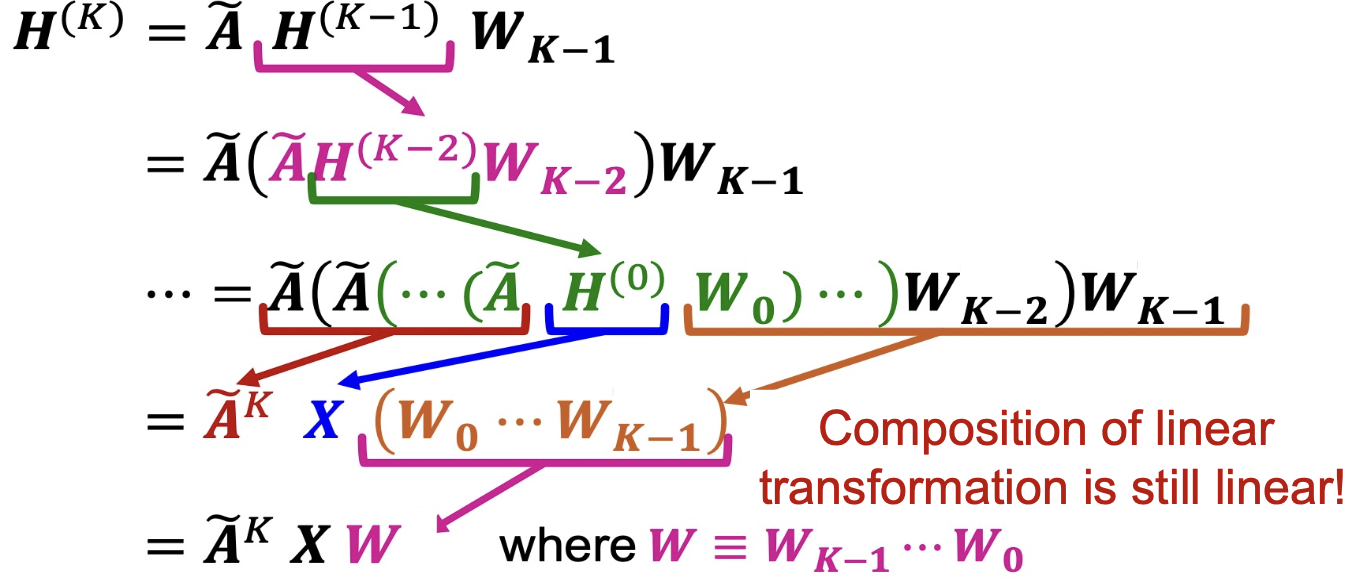
\includegraphics[height=0.06\textwidth]{figs/l9-1.png}  Notice that $\widetilde{X} = \widetilde{A}^KX$ contains no trainable parameter, so it can be pre-computed. Finally, implified GCN’s embedding is $H^{(K)} = \widetilde{X}W$, it’s just a linear transformation of precomputed matrix. For node $v$,its final embedding $h^k_v$ is $h^k_v=\widetilde{X}_vW$. \underline{Limitations}: Compared to the original GNN models, simplified GCN is less expressive as it removes the non-linearity. When does simplified GCN work? 1)Simplified GCN generates similar pre-processed features
for neighboring nodes. 2)Work well on homophilous graphs (neighboring nodes tend to share the same target labels). \hlorange{Distributed Learning}: Def: two or more machines collaborate on a single machine learning task. Require explicit (i.e. written in software) communication among the machines. \underline{Basic concepts}:\textbf{Push}: machine A sends some data to machine B. \textbf{Pull}: machine B requests some data from machine A. \textbf{All-Reduce}: compute some reduction (e.g., a sum) of data on multiple machines and synchronize the result on all those machines. \textbf{Data parallelism}: different machines have a complete copy of the model and a part of the data.\textbf{Model parallelism}: different machines are responsible for computation in different parts of a single model. \underline{Graph Partition} The input graph along with the features is partitioned across multiple machines. Partition schemes: random, edge-cut partitioner, or vertex-cut partitioner. \underline{Computation Graph Generation}Create the computation graph of each node in the mini- batch by pulling its k-hop neighborhood and the associated features. Require communication with other machines. \underline{Data Parallelism} Parallelize the mini-batch data on multiple machines and synchronize the gradients. \underline{Issue: Communication Bottleneck}: K-layer GNNs need to pull and aggregate the features of K- hop neighbors of nodes in each mini-batch training. Communication overhead dominates training time (GPUs are being underutilized).\underline{$P^3$} $P^3$ proposes push-pull parallelism for distributed GNNs that effectively eliminates the communication overhead. Key insights:1)The transmission of features causes dominant network traffic → avoiding feature movements.2)Existing system consider graph and features indivisible → independent partitioning of structure and features. \underline{$P^3$: Independent Partitioning}: Graph structure: partitioned using random scheme. pNode features: partitioned along feature dimension.\underline{$P^3$: Computation Graph Generation}Each machine samples a batch of nodes, then pulls the computational graph of each node. Features are not pulled, which reduces the network overhead of feature movement. Then, each machine pushes the locally created computational graphs to all other machines. \underline{$P^3$: Hybrid Parallelism} Model parallelism: each machine computes partial hidden node embeddings using the partial input features it owns. Each machine pulls the partial embeddings of nodes from other machines and aggregate them using reduce operation. GNNs typically use small hidden dimensions. The transmission of hidden embeddings incurs much less overhead compared to transferring original features. \underline{$P^3$: GNN training} Hybrid parallelism requires communication in forward and backward pass, which needs to pull partial hidden embeddings in the forward pass and push the gradients in the backward pass. \underline{$P^3$: Limitation}: It basically assumes the hidden dimension in GNNs is small. The benefits of $P^3$ decreases when increasing the number of hidden dimensions.


\hl{L10: AutoML on Graphs}
\hlgreen{AutoML}: Automated Machine Learning (AutoML) is the process of automating the tasks of applying machine learning to real-world problems. Neural Architecture Search (NAS) is a technique for automating the design of artificial neural networks. \hlgreen{AutoML on Graphs}: Two main directions: 1)Graph Neural Architecture Search (NAS), aimis to find the GNN architecture that can achieve the optimal performance on a given graph data 2) Hyper Parameter Optimization (HPO), aims to automatically find the optimal hyper-parameters of the GNN Model. \hlorange{Advantages of AutoML}: 1) Free humans out of the loop. 2) High optimization efficiency. 3)Discover and extract patterns and combinations automatically. \hlgreen{search space}: The search space in AutoGNN is differentiated according to GNN architectures and training hyperparameters. \underline{1)Micro-architecture:} To represent a graph convolutional layer,including \hlblue{hidden units} (feature dimensions, like 4,16,128), \hlblue{propagation} function (the function to compute the weight between nodes, like adjacency, GAT ...), \hlblue{aggregation func} (like SUM, MEAN, MAX), \hlblue{Combination func} (The function used to combine the embeddings of neighbors and node itselfs, like MLP), \hlblue{activation func} (ReLU, Sigmoid, Tanh, softmax...)\underline{2)Macro-architecture}: To represent network topology, including the \hlblue{layer depth}, \hlblue{inter-layer skip connections} e.g. [SUM, CAT, MAX, LSTM], and \hlblue{pre/post processing layers}. \underline{3) Hyperparameter}:\hlblue{drop out rate}, \hlblue{learning rate}, \hlblue{batchnorm} e.g. [False, BatchNorm, PairNorm,...], \hlblue{training epoch}. \hlgreen{Graph Neural Architecture Search}: includes Random Search, Evolutionary Search, Reinforcement Learning (RL) Based Search, Differentiable Search. \hlorange{Random Search} Given a search space, random search randomly samples the designs with equal probability. \hlorange{Evolutionary Search} \hlblue{Genetic Algorithm} reflects the process of natural selection, where the fittest individuals are selected for reproduction to produce offspring for the next generation. It contains these steps: 1. Initialize population (generate a series of GNN architectures). 2. Evaluate population (evaluate GNN architectures). 3. Select one GNN architecture as a parent. 4. Generate a new child architecture by applying mutations to it. \hlblue{Evolutionary Search Framework}: It contains these steps: 1.Randomly initialize the GNN structure population and parameter population. 2. Evolve parameters with structures fixed. 3. Evolve structures with parameters fixed. 4. Update structure and parameter population. \hlorange{Reinforcement Learning} It employs an RNN controller to sample an architecture. Then update the RNN controller based on the validation accuracy. Detailed process (s1: Generate a GNN architecture using controller RNN. s2: train on this setting and calculate the reward based on the performance. s3: Update controller. \hlorange{Differentiable Search} \hlblue{Goal}: Find the optimal GNN architecture that performs best on the specific task. \hlblue{Key idea}: Directly regard the entire search space as a supernet and learn how to sample an optimal subnet. Relax the search space to be continuous so that the architecture can be optimized concerning its validation set performance by gradient descent.\hlblue{Procedure} \hlblue{Step1: Initialization} Operations on the edges are initially unknown. The computation procedure for an architecture is represented as a directed acyclic graph (DAG). The cell indicates the different components that make up the GCN architecture, such as activation functions(sigmoid, ReLU...) Cell contains network weights. \hlblue{Step1: Relaxation of search space} Continuous relaxation of the search space by placing a mixture of candidate operations on each edge. The edges represent different operations of the GNN architecture components, such as sigmoid, ReLU. Edge contains its probability parameters. \hlblue{Joint-optimization} Joint optimization of the mixing probabilities and the network weights by solving a bilevel optimization problem. We will calculate the probability of operations on edges. Once the search progress terminates, the option with the highest probability is used in the final architecture \hlorange{Hyper Parameter Optimization
}: \hlblue{Goal} Automatically find the optimal hyper-parameter. \hlblue{Challenge}: Each trial of the inner loop on the graph is computationally expensive, especially for large-scale graphs. \hlorange{AutoNE}Goal: Transfer the knowledge about optimal hyper-parameters from sampled subgraphs to the original massive graph. \hlblue{Steps}: 1: Employ a \hlpurple{multi-start random walk strategy} to sample several small subgraphs. This stpe aims to sample representative subgraphs that share similar properties 2: Extract signature and perform each trial of configuration selection on the sampled subgraphs. This step aims to learn a vector representation for each subgraph so that knowledge can be transferred. This step uses NetLSD, builds on the Laplacian spectrum and preserves the community structure of a network.3: Design a Gaussian Process based meta-leaner to transfer the knowledge about optimal hyperparameters from the subgraphs to the original massive graph. This stpe aims to transfer knowledge about hyper-parameters of subgraphs to the original large-scale graph. It assumes similar graphs have similar optimal hyper- parameter.
 \hlorange{Two Phases of AutoNE} \hlblue{Phase I:Collect information} The goal of Phase I is to collect information about the performance function based on the results on the sampled subgraphs. \hlblue{Phase II: Predict the hyperparameters using meta learning.} In the phase II, the meta-learner makes $L$ predictions sequentially, where the results of the previous predictions will be leveraged to improve the next prediction.

\end{multicols*}
\end{document}